\documentclass[a4paper,10pt]{article}

\usepackage{subfig}
\usepackage{float}
\usepackage{graphicx}
\usepackage{verbatim}
\usepackage{amsthm}
\usepackage{amsmath}
\usepackage{amssymb}
\usepackage{geometry}
\usepackage[usenames,dvipsnames,svgnames,table]{xcolor}

\newtheorem{defn}{Definition}
\newtheorem{prop}{Proposition}
\newtheorem{theorem}{Theorem}

%opening
\title{Degree-dependent Rewiring Model}
\author{Sam Magura, Vitchyr Pong}

\begin{document}

\maketitle

\section{Model Definition}
The process operates on a graph $G = (V, E)$. Let $n$ be the number of vertices and let $m$ be the number of edges. Let
 \begin{equation}
f(i) = \theta \; (i + 1) + (1-\theta) \; (\overline{d} + 1),
\end{equation}
where $i$ is the degree of a vertex, $\overline{d}$ is the mean degree of the graph, and $\theta$ is a parameter.

\begin{prop}\label{prop:sum}
The sum of $f(i)$ over each vertex $w$ in the graph is given by
\begin{equation}
 \sum\limits_{w} f(d(w)) = 2m + n. 
 \end{equation}
\end{prop}
\begin{proof}
First, we note that

\begin{equation}
 \sum\limits_{w} f(d(w)) = \theta \left(\sum\limits_{w} d(w) + n\right) + (1-\theta)(n \,\overline{d} + n). 
 \end{equation}
 The sum of the degrees is equal to $2m$ by the handshaking theorem. The mean degree $\overline{d}$ is equal to $\frac{2m}{n}$. Therefore the RHS can be simplified to $\theta \left(2m + n\right) + (1-\theta)(2m + n) = 2m + n.$ 
\end{proof}

\paragraph{Procedure}
\begin{enumerate}
 \item Randomly select an edge from $E$.
 \item Select a random orientation $(x, y)$ for the edge.
 \item \label{item:z} Choose a vertex $z$ from $V$. Let the probability that some vertex $w$ is selected be
 
 \begin{equation}
 \label{eqn:pr}\frac{f(d(w))}{2m + n}.
 \end{equation} 

The denominator of this expression comes from the relationship
\begin{equation*}
 \sum\limits_{w} f(d(w)) = 2m + n, 
 \end{equation*}
which was proven in Proposition \ref{prop:sum}.

\item If $z$ is neither $x$ nor $y$, create an edge $\{x, z\}$ and remove the edge $\{x, y\}$.
\end{enumerate}

\section{Stationary Distribution}
The model is a Markov Chain because the probability of transitioning from a state $G$ to a state $H$ is dependent only $G$ and $H$. 

\begin{defn}
 Graphs $G = (V, E_G)$ and $H = (V, E_H)$ are the same state in the Markov Chain if and only if $E_G = E_H$.
\end{defn}


\paragraph{Transition probability} Consider states $G$ and $H$ such that $\{x, y\}$ is in $G$ but not $H$, and $\{x, z\}$ is in $H$ but not $G$. Let the degree of $y$ in $G$ be $j$ and the degree of $z$ in $H$ by $k$. Thus the degree of $y$ in $H$ is $j - 1$, and the degree of $z$ in $G$ is $k - 1$.
For a transition from $G$ to $H$, the following must occur.
\begin{enumerate}
 \item The edge $\{x, y\}$ is selected. This occurs with probability $\frac{1}{m}$.
 \item The orientation $(x, y)$ is chosen. This occurs with probability $\frac{1}{2}$.
 \item Vertex $z$ is selected in step \ref{item:z} of the model definition. This occurs with probability $\frac{f(k - 1)}{2m + n}$.
\end{enumerate}

\noindent Therefore the transition probability is 

\begin{equation}
\label{eqn:pgh}
 P(G, H) = \frac{1}{2m} \: \frac{f(k-1)}{2m+n}.
\end{equation}

\paragraph{Detailed balance}
Let 
\begin{equation}
 F(k) = \left\{
     \begin{array}{lr}
  \prod\limits_{i=0}^{k - 1} f(i) & : k \geq 1\\\\
  1 & : k = 0
     \end{array}
   \right..
\end{equation}
\begin{prop}\label{prop:F(k)}
 For an integer $k \geq 1$, $F(k - 1) \: f(k - 1) = F(k)$.
\end{prop}
\begin{proof}
When $k \geq 1$, $F(k - 1)$ expands to $f(0) \: f(1) \cdots f(k - 3) \: f(k - 2)$ and $F(k - 1) \: f(k - 1) = F(k)$. When $k = 1$, $F(k - 1) = F(0) = 1$ and $1 \cdot f(0) = F(1)$.
\end{proof}

\begin{theorem}
 The detailed balance condition is satisfied by the stationary distribution

\begin{equation}
 \pi(G) = c \prod_{w} F(d(w))
\end{equation}
where $c$ is some normalization coefficient.
\end{theorem}
\begin{proof}
The detailed balance condition is

\begin{equation}
 \pi(G) \: P(G, H) = \pi(H) \: P(H, G).
\end{equation}
Substituting in the transition probabilities from Equation \ref{eqn:pgh} and the proposed stationary distribution $\pi$, we have

\begin{equation}
\frac{1}{2m} \: \frac{f(k-1)}{2m+n}\:c\prod_{w \in G} F(d(w))  = \frac{1}{2m} \: \frac{f(j-1)}{2m+n}\:c\prod_{w \in H} F(d(w)).
\end{equation}
Recall that the only difference between $G$ and $H$ is that $G$ has an edge $\{x, y\}$ that $H$ does not and $H$ has an edge $\{x, z\}$ that $G$ does not. Thus we can reduce the previous equation to

\begin{equation}
F(k - 1) f(k - 1)\: F(j) = F(j - 1) \: f(j - 1) \: F(k).
\end{equation}
Because $k \geq 1$ and $j \geq 1$, we can apply Proposition \ref{prop:F(k)} to change $F(k - 1) \: f(k - 1)$ to $F(k)$ and $F(j - 1) \: f(j - 1)$ to $F(j)$. Therefore the detailed balance condition holds for the proposed stationary distribution $\pi$. 
\end{proof}

\section{Degree Distribution}
Let $N_k$ be the number of vertices in the graph that have degree $k$.
\begin{theorem}
\label{thm:exp-change}
The expected change in $N_k$ during an iteration is
\begin{equation*}
\label{eqn:N_k}
 \langle \Delta N_k \rangle = \frac{f(k - 1)}{2m + n} N_{k-1} + \frac{k + 1}{2m} N_{k + 1} - \frac{f(k)}{2m + n} N_{k} - \frac{k}{2m} N_{k}
\end{equation*}
for $k \geq 0$.
\end{theorem}
\begin{proof}
Consider the four ways in which $N_k$ can change during an iteration:
 \begin{enumerate}
 \item A vertex of degree $k - 1$ receives a new edge. $N_k$ increases by 1. This occurs with probability $\frac{f(k - 1)}{2m + n} N_{k-1}$ since the probability that a specific vertex of degree $k - 1$ is rewired to is $\frac{f(k - 1)}{2m + n}$ and there are $N_{k - 1}$ such vertices. This probability is trivially 0 for the $k = 0$ case, since there are no vertices of degree -1.
 
 \item A vertex of degree $k + 1$ has an incident edge removed. $N_k$ increases by 1. This occurs with probability $\frac{1}{2} \frac{k + 1}{m} N_{k + 1}$. For a specific vertex of degree $k + 1$ to have one of its $k + 1$ incident edges removed, this edge must first be selected; this occurs with probability $(k + 1)/ m$. Next, only one of the two possible orientations of this edge can result in the degree $k + 1$ vertex losing an edge. A vertex must also be chosen in Step \ref{item:z} of the procedure, but the probability that this occurs is nearly 1 for a large network.
 
 \item A vertex of degree $k$ receives a new edge. $N_k$ decreases by 1. This occurs with probability $\frac{f(k)}{2m + n} N_k$.
 
 \item A vertex of degree $k$ has an incident edge removed. $N_k$ decreases by 1. This occurs with probability $\frac{1}{2} \frac{k}{m} N_{k}.$ This probability is trivially 0 for the $k = 0$ case, since a vertex of degree 0 has no incident edges to be removed.
\end{enumerate}
We sum these probabilities to reach our final result. Probabilities for events that decrease $N_k$ by 1 are multiplied by -1.
\end{proof}

\begin{defn}
Let the stationary degree distribution be the degree distribution such that $\langle N_k \rangle = -$ for all $k \geq 0$. 
\end{defn}

\begin{theorem}
\label{thm:stationary-dd}
The stationary degree distribution is given by 
\begin{equation*}
\label{eqn:N_i}
 N_{i} = \frac{2m}{i}\left[\left( \frac{f(i - 1)}{2m + n} + \frac{i - 1}{2m} \right) N_{i - 1} -  \frac{f(i - 2)}{2m + n} N_{i - 2}\right].
\end{equation*}
for all $i \geq 1$.
\end{theorem}
\begin{proof}
 First we make the substitution $\langle N_k \rangle = 0$ in the relationship proved by Theorem \ref{thm:exp-change}. Now making the substitution $i = k + 1$, we get a recursive equation for the stationary degree distribution.
\end{proof}

The equation in Theorem \ref{thm:stationary-dd} can be simplified for the $i = 1$ case by noting that $N_{i - 2} = N_{-1} = 0$ and $\frac{i - 1}{2m} = 0$:
\begin{equation}
\label{eqn:N_1}
 N_{1} = \frac{2m}{2m + n} \; f(0) \; N_0.
\end{equation}
However, we still need a value for $N_0$ in order to caclualate $N_1, N_2,$ and so on. To solve this problem, we let $N_k = c \, M_k$ --- that is, let the sequence $M_0, M_1, M_2, \ldots$ be a sort of \emph{unnormalized} degree distribution. Next, we choose some arbitrary positive value for $M_0$, determine $M_1$ using Equation \ref{eqn:N_1}, and calculate all other $M_k$ values using Equation \ref{eqn:N_i}. For the normalization coefficient, we use
\begin{equation}
 c = \frac{n}{\sum\limits_{k=0}^{\infty} M_k}.
\end{equation}
This reflects the fact that, while $M_i / M_j = N_i / N_j$ for any $i$ and $j$, the sum $M_0 + M_1 + M_2 + \ldots$ probably does not sum to the total number of vertices $n$.
\definecolor{mygreen}{RGB}{12,170,0}
\begin{figure}
 \subfloat[$\theta=0.0$ \:\:\: $p=99.2\%$]{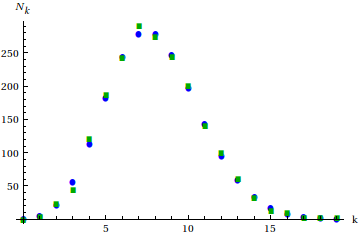
\includegraphics[width=7.0cm]{images/ddplot1.png}}
  \subfloat[$\theta=0.2$ \:\:\: $p=75.7\%$]{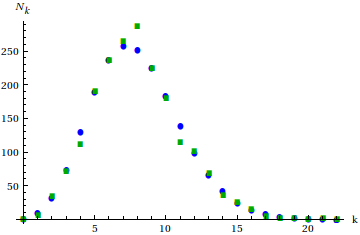
\includegraphics[width=7.0cm]{images/ddplot3.png}}\\\\
   \subfloat[$\theta=0.4$ \:\:\: $p=87.8\%$]{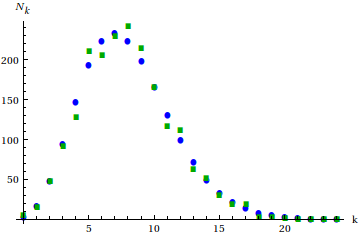
\includegraphics[width=7cm]{images/ddplot5.png}}
  \subfloat[$\theta=0.6$ \:\:\: $p=93.7\%$]{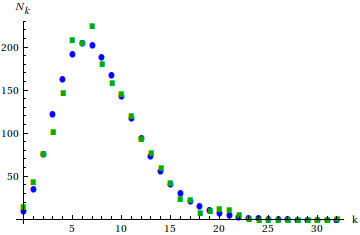
\includegraphics[width=7cm]{images/ddplot7.png}}\\\\
   \subfloat[$\theta=0.8$ \:\:\: $p=95.8\%$]{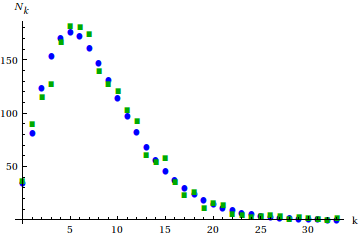
\includegraphics[width=7cm]{images/ddplot9.png}}
  \subfloat[$\theta=1.0$ \:\:\: $p=99.6\%$]{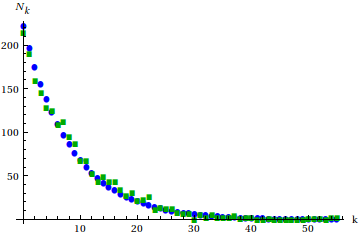
\includegraphics[width=7cm]{images/ddplot11.png}}
  \caption{Comparison of expected (\color{blue}{\textbullet}\color{black}) and observed (\tiny\color{mygreen}$\blacksquare$\color{black}\normalsize) stationary degree distributions. Note the different scales on the axes of each plot. A graph with 2000 vertices and 8000 edges was used in each trial. For $\theta = 0.0 \ldots 0.8$, 100,000 iterations were performed. For the $\theta=1.0$ case, more iterations (200,000) were required to reach the stationary degree distribution, presumably because it is so different from the degree distribution of the original $G(n,m)$ random graph.}
  \label{fig:dd}
\end{figure}

\subsection{Comparison to observed degree distribution} 
We implemented the model in C using the igraph library. The program constructs a $G(n, m)$ random graph and then performs a specified number of iterations on that graph. Finally, the program reports the degree distribution of the final graph. For a large graph and a sufficient number of iterations, this observed degree distribution should match our predictions for the stationary degree distribution. We ran $\chi^2$--tests to quantify the goodness-of-fit. When doing this, we did not compare the expected and observed frequencies of a certain degree if either frequency was less than 5, because the $\chi^2$--test is not valid for such low frequencies. Figure \ref{fig:dd} shows the expected and observed degree distributions as well as the corresponding $p$-values. Prediction and experiment matched very well for every value of $\theta$ tested --- each $p$-value was well above the commonly used significance level of $5\%$.

\subsection{Discussion and additional analysis}

\begin{theorem}
 When $\theta=0$, the stationary degree distribution is Poisson. Specifically,
 \begin{equation}
  N_i = n \;\frac{\lambda^i \, e^{-\lambda}}{i!} \mbox{\;\;\;\;with\;\;\;\;} \lambda = \frac{2m}{2m+n}\,(\overline{d} + 1).
 \end{equation}
 \end{theorem}
\begin{proof}
 A random variable $X$ has a Poisson distribution if
 \begin{equation}
  Pr(X=i)=\frac{\lambda^i\;e^{-\lambda}}{i!}.
 \end{equation}
In this case, $X = d(w)$ where $w$ is a vertex selected randomly from the graph. Therefore $Pr(X=i)=\frac{N_i}{n}$.\\\\
Let $P_i$ be the statement that $N_i = \frac{\lambda}{i} \; N_{i - 1}$ where $\lambda = \frac{2m}{2m+n}\,(\overline{d} + 1).$ We begin by proving $P_i$ for all $i \geq 1$ using induction.
\paragraph{Basis}
When $\theta=0$, $f(i) = \overline{d} + 1.$ With this, we can see that $P_1$ is true by Equation \ref{eqn:N_1}.
\paragraph{Inductive step} Assume $P_{i - 1}$ is true; that is, that $N_{i - 1} = \frac{\lambda}{i - 1} \; N_{i - 2}$. Substite $\frac{i - 1}{\lambda} \; N_{i - 1}$ for $N_{i - 2}$ and $\overline{d} + 1$ for $f(i)$ in Equation \ref{eqn:N_i} to get
\begin{equation}
 N_{i} = \frac{2m}{i}\left[\left( \frac{\overline{d}+1}{2m + n} + \frac{i - 1}{2m} \right) N_{i - 1} - \frac{\overline{d}+1}{2m + n} \left( \frac{i - 1}{\overline{d} + 1} \; \frac{2m + n}{2m} \right) N_{i - 1}\right].
\end{equation}
After simplification, this reduces to
\begin{equation}
 N_i = \frac{2m}{2m+n}\,\frac{\overline{d} + 1}{i} \; N_{i - 1} = \frac{\lambda}{i} \;N_{i - 1}
\end{equation}
and $P_i$ holds. By the principle of mathematical induction, $P_i$ holds for all $i \geq 1.$
\\\\
We have shown that $N_i = \frac{\lambda^i}{i!} \; N_0$ for all $i \geq 1$, but $N_0$ remains unknown. By recognizing that $N_0 + N_1 + N_2 + \ldots = n$, we can write the equation
\begin{equation}
 N_0 \sum\limits_{i=0}^\infty \frac{\lambda^i}{i!} = n.
\end{equation}
This infinite series is the Maclaurin series for $e^\lambda$. Thus $N_0 = n\, e^{-\lambda}$, and $N_i = n \,\frac{\lambda^i \, e^{-\lambda}}{i!}$ for all $i \geq 0$.

\end{proof}


\begin{theorem}
 For $\theta=1$, the stationary degree distribution is given by an exponential function
 \begin{equation}
  N_i = N_0 \left(\frac{2m}{2m + n}\right)^i.
 \end{equation}
\end{theorem}
\begin{proof}
Proceed by induction. Let $P_i$ be the statement that $N_i = N_0 (\frac{2m}{2m+n})^i$.
\paragraph{Basis}
$P_0$ is trivially true. To prove $P_1$, we first note that when $\theta=1$, $f(i) = i + 1.$ Using this, we can simplify Equation \ref{eqn:N_1} to
 \begin{equation}
  N_{1} = \frac{2m}{2m + n} \; N_0.
 \end{equation}
$P_1$ is true.
\paragraph{Inductive step}
Assume statements $P_{i-2}$ and $P_{i-1}$ are true. Now we rewrite Equation \ref{eqn:N_i} for the special case when $\theta = 1$:
\begin{equation}
N_{i} = \frac{2m}{i}\left[\left( \frac{i}{2m + n} + \frac{i - 1}{2m} \right) N_{i - 1} -  \frac{i - 1}{2m + n} N_{i - 2}\right].
\end{equation}
Since we are assuming $P_{i-2}$ and $P_{i-1}$, we know that $N_{i - 1} = \frac{2m}{2m + n} N_{i - 2}$. From this relationship, we can make the substitution $N_{i - 2} = \frac{2m + n}{2m} N_{i - 1}$:
\begin{equation}
N_{i} = \frac{2m}{i}\left( \frac{i}{2m + n} + \frac{i - 1}{2m} - \frac{2m + n}{2m} \; \frac{i - 1}{2m + n}\right) N_{i - 1}.
\end{equation}
After simplifying, we find that $P_i$ holds. By the principle of mathematical induction, $P_i$ holds for all $i \geq 0$.

\end{proof}


\end{document}
